\documentclass[tikz,border=2pt]{standalone}
\usepackage{amsmath}
\usepackage{tikz}
\usetikzlibrary{arrows.meta}

\begin{document}
% |x+y| <= |x| + |y|: on the number line the step x followed by the step y never lands further
% from 0 than |x|+|y|; equality only when x and y point the same way.
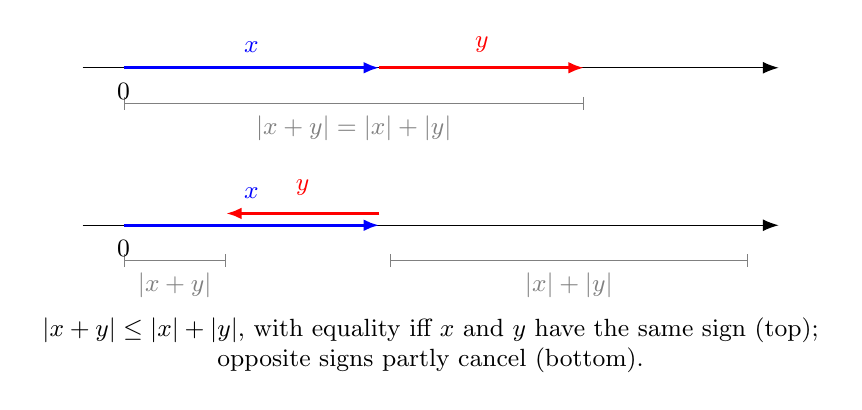
\begin{tikzpicture}[x=1.3cm, every node/.style={font=\small}]
	% case 1: same sign
	\draw[-{Latex[length=2mm]}] (-0.4,1.6) -- (6.4,1.6);
	\draw[blue, very thick, -{Latex[length=2mm]}] (0,1.6) -- (2.5,1.6);
	\draw[red, very thick, -{Latex[length=2mm]}] (2.5,1.6) -- (4.5,1.6);
	\node[blue, above=2pt] at (1.25,1.6) {$x$};
	\node[red, above=2pt] at (3.5,1.6) {$y$};
	\draw[gray, |-|] (0,1.15) -- (4.5,1.15);
	\node[gray, below=1pt] at (2.25,1.15) {$|x+y|=|x|+|y|$};
	\node[below=2pt] at (0,1.6) {$0$};
	% case 2: opposite signs
	\draw[-{Latex[length=2mm]}] (-0.4,-0.4) -- (6.4,-0.4);
	\draw[blue, very thick, -{Latex[length=2mm]}] (0,-0.4) -- (2.5,-0.4);
	\draw[red, very thick, -{Latex[length=2mm]}] (2.5,-0.25) -- (1.0,-0.25);
	\node[blue, above=6pt] at (1.25,-0.4) {$x$};
	\node[red, above=3pt] at (1.75,-0.25) {$y$};
	\draw[gray, |-|] (0,-0.85) -- (1.0,-0.85);
	\node[gray, below=1pt] at (0.5,-0.85) {$|x+y|$};
	\draw[gray, |-|] (2.6,-0.85) -- (6.1,-0.85);
	\node[gray, below=1pt] at (4.35,-0.85) {$|x|+|y|$};
	\node[below=2pt] at (0,-0.4) {$0$};
	\node[anchor=north, align=flush center, text width=10cm] at (3,-1.45) {$|x+y|\le |x|+|y|$, with equality iff $x$ and $y$ have the same sign (top); opposite signs partly cancel (bottom).};
\end{tikzpicture}
\end{document}
